\documentclass[a4paper,12pt]{article}

%%% Работа с русским языком
\usepackage{cmap}					% поиск в PDF
\usepackage{mathtext} 				% русские буквы в формулах
\usepackage[T2A]{fontenc}			% кодировка
\usepackage[utf8]{inputenc}			% кодировка исходного текста
\usepackage[english,russian]{babel}	% локализация и переносы
\usepackage{indentfirst}            % красная строка в первом абзаце
\usepackage{extarrows}              % длинное равно
\frenchspacing                      % равные пробелы между словами и предложениями

%%% Дополнительная работа с математикой
\usepackage{amsmath,amsfonts,amssymb,amsthm,mathtools} % пакеты AMS
\usepackage{icomma}                                    % "Умная" запятая
\usepackage{physics} % для символа нормы

%%% Свои символы и команды
\usepackage{centernot} % центрированное зачеркивание символа
\usepackage{stmaryrd}  % некоторые спецсимволы

\usepackage{pythonhighlight}

% \renewcommand{\epsilon}{\ensuremath{\varepsilon}}
% \renewcommand{\phi}{\ensuremath{\varphi}}
% \renewcommand{\kappa}{\ensuremath{\varkappa}}
% \renewcommand{\le}{\ensuremath{\leqslant}}
% \renewcommand{\leq}{\ensuremath{\leqslant}}
% \renewcommand{\ge}{\ensuremath{\geqslant}}
% \renewcommand{\geq}{\ensuremath{\geqslant}}
% \renewcommand{\emptyset}{\ensuremath{\varnothing}}

% \DeclareMathOperator*{\Mid}{\scalebox{1.1}{$\mid$}}
\DeclareMathOperator*{\argmax}{argmax}

% \DeclareMathOperator{\sgn}{sgn}
% \DeclareMathOperator{\gd}{\text{НОД}}
% \DeclareMathOperator{\lf}{\text{НОК}}
% \DeclareMathOperator{\rk}{rk}
% \DeclareMathOperator{\pr}{pr}
% \DeclareMathOperator{\im}{Im}
% \DeclareMathOperator{\ke}{Ker}
% \DeclareMathOperator{\re}{Re}
% \DeclareMathOperator{\cha}{char}
% \DeclareMathOperator{\ord}{ord}
% \DeclareMathOperator{\tr}{tr}
% \DeclareMathOperator{\md}{mod}
% \DeclareMathOperator{\Aut}{Aut}
% \DeclareMathOperator{\Inn}{Inn}
% \DeclareMathOperator{\End}{End}
% \DeclareMathOperator{\GL}{GL}
% \DeclareMathOperator{\SL}{SL}
% \DeclareMathOperator{\diag}{diag}

\newcommand{\divby}{
	\mathrel{\vbox{\baselineskip.65ex\lineskiplimit0pt\hbox{.}\hbox{.}\hbox{.}}}
}
\newcommand{\notdivby}{\centernot\divby}
% \newcommand\norm[1]{\left\lVert#1\right\rVert}
% \newcommand\normx[1]{\left\Vert#1\right\Vert}
\newcommand{\N}{\mathbb{N}}
\newcommand{\Z}{\mathbb{Z}}
\newcommand{\Q}{\mathbb{Q}}
\newcommand{\R}{\mathbb{R}}
\newcommand{\E}{\mathbb{E}}
\newcommand{\D}{\mathbb{D}}
\newcommand{\Cm}{\mathbb{C}}
\newcommand{\F}{\mathbb{F}}
\newcommand{\id}{\mathrm{id}}
\newcommand{\imp}[2]{(#1\,\,$\ra$\,\,#2)\,\,}
\newcommand{\nset}[1]{\{1, \dotsc, #1\}}
\newcommand{\Chi}{\scalebox{1.1}{\raisebox{\depth}{$\chi$}}}
\newcommand{\FF}{\scalebox{0.95}{$\mathcal F$}}
\newcommand{\FFF}{\scalebox{0.55}{$\mathcal F$}}
\newcommand{\GG}{\scalebox{0.95}{$\mathcal G$}}
\newcommand{\GGG}{\scalebox{0.55}{$\mathcal G$}}

\newcommand{\ND}[2]{\mathcal{N}\left({#1}, {#2}\right)} % normal distribution
\newcommand{\tod}{\xrightarrow[]{d}}
\newcommand{\toP}{\xrightarrow[]{P}}
\newcommand{\tolp}[1]{\xrightarrow[]{L_{#1}}}
\newcommand{\toac}{\xrightarrow[]{\text{п. н.}}} % almost certainly

\renewcommand\labelitemi{$\triangleright$}
\newcommand{\LL}{\mathcal{L}}
\newcommand{\todo}[1]{\textcolor{red}{TODO} #1}
\let\bs\backslash
\let\vect\overline
\let\normal\trianglelefteqslant
\let\lra\Leftrightarrow
\let\ra\Rightarrow
\let\la\Leftarrow
\let\gl\langle
\let\gr\rangle
\let\sd\leftthreetimes
\let\emb\hookrightarrow
\let\mc\mathcal
\let\mf\mathfrak

%%% Перенос знаков в формулах (по Львовскому)
\newcommand*{\hm}[1]{#1\nobreak\discretionary{}{\hbox{$\mathsurround=0pt #1$}}{}}
\renewcommand{\phi}{\varphi}
\newcommand{\eps}{\varepsilon}

%%% Работа с картинками
\usepackage{graphicx}    % Для вставки рисунков
\setlength\fboxsep{3pt}  % Отступ рамки \fbox{} от рисунка
\setlength\fboxrule{1pt} % Толщина линий рамки \fbox{}
\usepackage{wrapfig}     % Обтекание рисунков текстом

%%% Работа с таблицами
\usepackage{array,tabularx,tabulary,booktabs} % Дополнительная работа с таблицами
\usepackage{longtable}                        % Длинные таблицы
\usepackage{multirow}                         % Слияние строк в таблице

%%% Теоремы
\theoremstyle{definition}
\newtheorem{problem}{}
\newtheorem{theorem}{Теорема}
\newtheorem*{lemma}{Лемма}
% \newtheorem{proposition}{Утверждение}[section]
% \newtheorem*{exercise}{Упражнение}
% \newtheorem{problem}{}

% \theoremstyle{definition}
% \newtheorem{definition}{Определение}[section]
% \newtheorem*{corollary}{Следствие}
% \newtheorem*{note}{Замечание}
% \newtheorem*{reminder}{Напоминание}
% \newtheorem*{example}{Пример}

\theoremstyle{remark}
\newtheorem*{solution}{Решение}
\newtheorem*{guidance}{Указание}
\newtheorem*{prooff}{Д-во}

%%% Оформление страницы
\usepackage{extsizes}     % Возможность сделать 14-й шрифт
\usepackage{geometry}     % Простой способ задавать поля
\usepackage{setspace}     % Интерлиньяж
\usepackage{enumitem}     % Настройка окружений itemize и enumerate
\setlist{leftmargin=25pt} % Отступы в itemize и enumerate

\geometry{top=25mm}    % Поля сверху страницы
\geometry{bottom=30mm} % Поля снизу страницы
\geometry{left=20mm}   % Поля слева страницы
\geometry{right=20mm}  % Поля справа страницы

\setlength\parindent{15pt}                % Устанавливает длину красной строки 15pt
\linespread{1.3}                          % Коэффициент межстрочного интервала
%\setlength{\abovedisplayskip}{3pt}       % Отступы от выключных формул
%\setlength{\belowdisplayskip}{3pt}       % Отступы от выключных формул
%\setlength{\abovedisplayshortskip}{3pt}  % Отступы от выключных формул
%\setlength{\abovedisplayshortskip}{3pt}  % Отступы от выключных формул
%\setlength{\parskip}{0.5em}              % Вертикальный интервал между абзацами
%\setcounter{secnumdepth}{0}              % Отключение нумерации разделов
%\setcounter{section}{-1}                 % Нумерация секций с нуля
\usepackage{multicol}			          % Для текста в нескольких колонках
\usepackage{soulutf8}                     % Модификаторы начертания

%%% Содержаниие
\usepackage{tocloft}
\renewcommand{\thesection}{\arabic{section}.} 
\renewcommand{\thesubsection}{\thesection.\arabic{subsection}.}
\tocloftpagestyle{main}
%\setlength{\cftsecnumwidth}{2.3em}
%\renewcommand{\cftsecdotsep}{1}
%\renewcommand{\cftsecpresnum}{\hfill}
%\renewcommand{\cftsecaftersnum}{\quad}

%%% Шаблонная информация для титульного листа
\newcommand{\CourseName}{Математическая статистика}
\newcommand{\FullCourseName}{\so{МАТЕМАТИЧЕСКАЯ СТАТИСТИКА}}
\newcommand{\TaskNumber}{II}
\newcommand{\CourseDate}{весна 2024}
\newcommand{\AuthorInitials}{Яфаров Руслан}

%%% Колонтитулы
% \usepackage{titleps}
% \newpagestyle{main}{
% 	\setheadrule{0.4pt}
% 	\sethead{\CourseName}{}{\hyperlink{intro}{\;Назад к содержанию}}
% 	\setfootrule{0.4pt}                       
% 	\setfoot{ФПМИ МФТИ, \CourseDate}{}{\thepage} 
% }
% \pagestyle{main}  

%%% Нумерация уравнений
\makeatletter
\def\eqref{\@ifstar\@eqref\@@eqref}
\def\@eqref#1{\textup{\tagform@{\ref*{#1}}}}
\def\@@eqref#1{\textup{\tagform@{\ref{#1}}}}
\makeatother                      % \eqref* без гиперссылки
\numberwithin{equation}{section}  % Нумерация вида (номер_секции).(номер_уравнения)
\mathtoolsset{showonlyrefs=false} % Номера только у формул с \eqref{} в тексте.

%%% Гиперссылки
\usepackage{hyperref}
% \usepackage[usenames,dvipsnames,svgnames,table,rgb]{xcolor}
\hypersetup{
	unicode=true,            % русские буквы в раздела PDF
	colorlinks=true,       	 % Цветные ссылки вместо ссылок в рамках
	linkcolor=black!15!blue, % Внутренние ссылки
	citecolor=green,         % Ссылки на библиографию
	filecolor=magenta,       % Ссылки на файлы
	urlcolor=NavyBlue,       % Ссылки на URL
}

%%% Графика
\usepackage{tikz}        % Графический пакет tikz
\usepackage{tikz-cd}     % Коммутативные диаграммы
\usepackage{tkz-euclide} % Геометрия
\usepackage{stackengine} % Многострочные тексты в картинках

\begin{document}
	\begin{titlepage}
	\clearpage\thispagestyle{empty}
	\centering
	
	\textbf{Московский физико-технический институт}
	\vspace{33ex}
	
	{\textbf{\FullCourseName}}
	
	\TaskNumber\ ЗАДАНИЕ 
	\vspace{1ex}

	\begin{flushright}
		\noindent
		Автор: {\AuthorInitials},
		\\
		Б13-202 
	\end{flushright}
	
	\vfill
	\CourseDate
	\pagebreak
\end{titlepage}
	\section{Байесовские оценки}
  \problem{
  $X_1 \sim Exp(\theta)$, $\theta$ имеет сопряженное априорное распределение $\Gamma(\alpha, \beta)$. Проверьте оценку $\theta^* = \frac{n + \beta}{\alpha + \sum_{i = 1}^n X_i}$ на состоятельность.
  }
  \solution{}
  \problem{
  По выборке $X_1, \dots, X_n$ из пуассоновского распределения с параметром $\theta$, где $\theta \sim \Gamma(\alpha, \lambda)$, постройте наилучшую оценку в байесовском подходе с квадратичной функцией потерь.
  }
  \solution{}
  \problem{
  Пусть $X_1, \dots, X_n$ - выборка из нормального распредения с параметрами $(\theta, 1)$. Найдите байесовскую оценку параметра $\theta$, если априорное распределение $\theta$ есть $Bin(1, p)$. Будет ли полученная оценка состоятельной оценкой параметра $\theta$?
  }
  \solution{}
  \problem{
  Пусть $X_1, \dots, X_n$ - выборка из равномерного распределения на отрезке $[0, \theta]$. Найдите байесовскую оценку параметра $\theta$, если $\theta$ имеет априорное распределение а) равномерно на отрезке $[0, 1]$, б) с плотностью $q(t) = 1/t^2$ при $t \ge 1$. Проверьте полученные оценки на состоятельность.
  }
  \solution{}
  \problem{
  Пусть $X_1, \dots, X_n$ - выборка из нормального распределения с параметрами $(\theta, 1)$. Найдите байесовскую оценку параметра $\theta$, если априорное распределение $\theta$ есть $\ND{b}{\sigma^2}$.}
  \solution{~}
  \section{Проверка гипотез и доверительное оценивание}
  \problem{
  $X_1, \dots, X_n$ - выборка из распределения с плотностью
  \[p_{\theta}(x) = \frac{3x^2}{8\theta^3}I_{[0, 2\theta]}(x)\]
  С помощью статистики $X_{(1)}$ постройте точный доверительный интервал уровня доверия $\gamma$ для параметра $\theta$.
  }
  \solution{
  $F_{X_{(1)}}(x) = 1 - (1 - F_{X_1}(x))^n = 1 - (1 - \frac{x^3}{8\theta^3})^n, x \in [0, 2\theta] \ra F_{\frac{X_{(1)}}{2\theta}}(x) = F_{X_{(1)}}(2\theta x) = 1 - (1 - x^3)^n, x \in [0, 1]$.
  \[P_{\theta}\left(z_{p_1} < \frac{X_{(1)}}{2\theta} < z_{p_2}\right) = P_{\theta}\left(\frac{X_{(1)}}{2z_{p_2}} < \theta < \frac{X_{(1)}}{2z_{p_1}}\right) = p_2 - p_1 = \gamma \]
  Положим $p_2 = 1, p_1 = 1 - \gamma$, тогда $z_{p_2} = 1, z_{p_1} = \sqrt[3]{1 - \sqrt[n]{\gamma}}$\\
  Ответ: $\left(\frac{X_{(1)}}{2}, \frac{X_{(1)}}{2\sqrt[3]{1 - \sqrt[n]{\gamma}}}\right)$
  }
  \problem{
  $X_1, \dots, X_n$ - выборка, $X_1 = \xi + \eta$, где $\xi$, $\eta$ - независимые случайные величины, $\xi \sim R[0, \theta], \eta \sim Bin(1, \theta)$. Постройте доверительный интервал для $\theta$ уровня доверия $1 - \alpha $ с помощью неравенства Чебышева.
  }
  \solution{
  $\E X_1 = \E \xi + \E \eta = \theta/2 + \theta = \frac{3\theta}{2}, \D X_1 = \D \xi + \D \eta = \frac{\theta^2}{12} + \theta(1 - \theta) = \theta - \frac{11}{12}\theta^2$
  \[P_{\theta}\left(\left|\sum_{i = 1}^n X_i - \frac{3\theta n}{2}\right| \ge \eps n\right) \le \frac{\theta - \frac{11}{12}\theta^2}{\eps^2n} \ra P_{\theta}\left(\overline{X} - \eps < \frac{3\theta}{2} < \overline{X} + \eps\right) \ge 1 - \frac{\theta - \frac{11}{12}\theta^2}{\eps^2n} = 1 - \alpha \ra 
  \]
  \[
  \eps = \sqrt{\frac{\theta - \frac{11}{12}\theta^2}{\alpha n}}, \text{ Получаем } 
  \begin{cases}
  \overline{X} - \frac{3\theta}{2} < \eps, \\
  \overline{X} - \frac{3\theta}{2} > -\eps
  \end{cases} \lra 
  \left(\overline{X} - \frac{3\theta}{2} \right)^2 < \eps^2 \lra \] \[
  \theta^2 \left(\frac{9}{4} + \frac{11}{12\alpha n}\right) - \theta \left(3\overline{X} + \frac{1}{\alpha n}\right) + \overline{X}^2 < 0 \ra
  \]
  \[
  \text{Ответ: } \left(\frac{3\overline{X} + \frac{1}{\alpha n} - \sqrt{\left(3\overline{X} + \frac{1}{\alpha n}\right)^2 - 4\left(\frac{9}{4} + \frac{11}{12\alpha n}\right)\overline{X}^2}}{2\left(\frac{9}{4} + \frac{11}{12\alpha n}\right)}, \frac{3\overline{X} + \frac{1}{\alpha n} + \sqrt{\left(3\overline{X} + \frac{1}{\alpha n}\right)^2 - 4\left(\frac{9}{4} + \frac{11}{12\alpha n}\right)\overline{X}^2}}{2\left(\frac{9}{4} + \frac{11}{12\alpha n}\right)} \right)
  \]
  }
  \problem{
  Пусть $X_1, \dots, X_n$ - выборка из гамма-распределения с параметрами $(\theta, \lambda)$. Постройте асимптотический доверительный интервал для $\theta$ уровня доверия $\alpha$, если а) $\lambda$ известно, б) $\lambda$ неизвестно.
  }
  \solution{~
  \begin{enumerate}[label=\alph*]
  \item По ЦПТ $\sqrt{n}(\overline{X} - \lambda \theta) \tod \ND{0}{\theta \lambda^2}$
  Пусть $z_p $ - квантиль уровня $p$ распределения $\ND{0}{1}$. Так как $\lambda\sqrt{\theta}$ непрерывна по $\theta$ на $\R_{+}$, то
  \[\lim_{n \to \infty} P\left(z_{\frac{1 - \alpha}{2}} < \sqrt{n} \frac{\overline{X} - \lambda \theta}{\lambda \sqrt{\overline{X}}} < z_{\frac{1 + \alpha}{2}}\right) = \alpha\]
  Ответ: $\left(\frac{\overline{X} - \frac{z_{\frac{1 + \alpha}{2}}\lambda \sqrt{\overline{X}}}{\sqrt{n}}}{\lambda}, \frac{\overline{X} - \frac{z_{\frac{1 - \alpha}{2}}\lambda \sqrt{\overline{X}}}{\sqrt{n}}}{\lambda}\right)$
  \end{enumerate}
  }
  \problem{
  Имеется $X_1$ - выборка объема 1. Основная гипотеза $H_0$ состоит в том, что $X_1$ имеет равномерное распределение на отрезке $[0, 1]$, альтернатива - в том, что $X_1$ имеет показательное распределение с параметром 1. Постройте наиболее мощный критерий уровня значимости $\alpha$ для различения этих гипотез и вычислите его мощность.
  }
  \solution{}
  \problem{
  Пусть $X_1, \dots, X_n$ - выборка из равномерного распределения на отрезке $[0, \theta], \theta > 0$. Постройте р.н.м.к. уровня значимости $\alpha$ для проверки гипотезы $H_0 : \theta = \theta_0$ против альтернативы $H_1: \theta \ne \theta_0$ в виде
\[S(X_1, \dots, X_n) = \{ X_{(n)} \le c\theta_0\} \cup \{ X_{(n)} > \theta_0 \}\]
  }
  \solution{}
  \problem{
  Пусть $\{P_{\theta}, \theta \in \Theta\}$ - семейство с невозрастающим отношением правдоподобия по статистике $T(X)$, а $\alpha < 1$ - некоторое положительное число. Постройте р.н.м.к. уровня значимости $\alpha$ для проверки гипотезы $H_0$ против альтернативы $H_1$ , где а) $H_0 : \theta \le \theta_0$ (или $\theta = \theta_0), H_1 : \theta > \theta_0 $;
б) $H_0 : \theta \ge \theta_0$ (или $\theta = \theta_0$ ), $H_1 : \theta < \theta_0$ .
  }
  \solution{}
  \problem{*
  Показать, что любой равномерно наиболее мощный несмещённый (т.е. $\inf_{\theta \in \Theta_0} \beta(\theta, S) \ge \sup_{\theta \in \Theta_1} \beta(\theta, S)$) критерий $S$ является допустимым, т.е. не существует другого критерия $R$, который был бы не менее мощен, чем $S$, при всех альтернативах и более мощен хотя бы при одной из альтернатив.}
  \solution{}
  \problem{
  Докажите, что в предположении гипотезы $H_0 : F = F_0$ для любого $x \in R$ выполнено
\[ F_n^*(x) \xrightarrow[n \to \infty]{\text{п. н.}} F_0(x)\]
  }
  \solution{}
  \begin{theorem}[А. Колмогорова, 12.2 из С2]
  В предположении верности гипотезы $H_0 : F = F_0$ имеет место равенство 
  \[\lim_{n \to \infty} P(\sqrt{n}D_n \le t) = K(t)\]
  \end{theorem}
  \problem{
  С помощью теоремы 1 докажите состоятельность критерия Колмогорова.

  }
  \solution{}
  \problem{
  Докажите, что при условии $0 \le X_{(1)} \le X_{(n)} \le 1$ справедливо равенство
\[\int_{0}^1 (F_n^*(y) - y)^2dy = \frac{1}{12n^2} + \frac{1}{n} \sum_{k = 1}^n (X_{(k)} - (2k - 1) / 2n)^2 \]
(с помощью этого представления часто вычисляется значение статистики $\omega^2$ , которая используется в критерии
Крамера–Мизеса–Смирнова).
  }
  \solution{}
  \problem{
  Цифры $0, 1, 2, \dots , 9$ среди $800$ первых десятичных знаков
числа $\pi$ появились \\$74, 92, 83, 79, 80, 73, 77, 75, 76, 91$ раз соответственно. С помощью хи-квадрат критерия проверьте гипотезу о согласии этих данных с законом равномерного распределения на множестве $\{0, 1, \dots , 9\}$ на уровне
значимости а) 0.05, б) 0.5, в) 0.8.
}
  \solution{}
  \problem{
  Среди $5000$ семей, имеющих трех детей, есть ровно $1010$ семей с тремя мальчиками, 2200 семей с двумя мальчиками и одной девочкой, 950 семей с одним мальчиком и двумя девочками (во всех остальных семьях все дети - девочки). Можно ли с уровнем значимости $\alpha = 0.02$ считать, что количество мальчиков $\xi$ в семье с тремя детьми имеет следующее распределение
\[
P(\xi = 0) = \theta, P(\xi = 1) = \theta, \]
\[P(\xi = 2) = 2\theta, P(\xi = 3) = 1 - 4\theta, \]
где $\theta \in (0, 1/4)$?
  }
  \solution{}
  \problem{
  Пусть $X_1, \dots, X_n$ - выборка из распределения:
а)$Bern(\theta)$, б)$Pois(\theta)$, в)$\ND{\theta}{1}$, г)$\exp(\theta)$.
Построить доверительный интервал для параметра $\theta$.
  }
  \solution{
  Будем строить доверительные интервалы уровня доверия $\gamma = 1 - \alpha$
  \begin{enumerate}[label=\alph*]
  \item 
  \[P_{\theta}\left(\left|\sum_{i = 1}^n X_i - \theta n \right| \ge \eps n\right) \le \frac{\theta(1 - \theta)}{\eps^2n} \ra P_{\theta}\left(\overline{X} - \eps < \theta < \overline{X} + \eps\right) \ge 1 - \frac{\theta(1 - \theta)}{\eps^2n} = 1 - \alpha \ra 
  \]
  \[
  \eps = \sqrt{\frac{\theta(1 - \theta)}{\alpha n}}, \text{ Получаем } 
  \left(\overline{X} - \theta \right)^2 < \eps^2 \lra 
  \theta^2 \left(1 + \frac{1}{\alpha n}\right) - \theta \left(2\overline{X} + \frac{1}{\alpha n}\right) + \overline{X}^2 < 0 \ra
  \]
  \[
  \text{Ответ: }\left(\frac{2\overline{X} + \frac{1}{\alpha n} - \sqrt{\left(2\overline{X} + \frac{1}{\alpha n}\right)^2 - 4\left(1 + \frac{1}{\alpha n}\right)\overline{X}^2}}{2\left(1 + \frac{1}{\alpha n}\right)}, \frac{2\overline{X} + \frac{1}{\alpha n} + \sqrt{\left(2\overline{X} + \frac{1}{\alpha n}\right)^2 - 4\left(1 + \frac{1}{\alpha n}\right)\overline{X}^2}}{2\left(1 + \frac{1}{\alpha n}\right)} \right)
  \]
  \item По аналогии с предыдущей задачей, $\E X = \theta, \D X = \theta$, получаем неравенство $\theta^2 - \theta\left(2\overline{X} + \frac{1}{\alpha}\right) + \overline{X}^2 < 0 \ra$
  \[\text{Ответ: } \left(\frac{2\overline{X} + \frac{1}{\alpha} + \sqrt{\frac{4\overline{X}}{\alpha} + \frac{1}{\alpha^2}}}{2}, \frac{2\overline{X} + \frac{1}{\alpha} - \sqrt{\frac{4\overline{X}}{\alpha} + \frac{1}{\alpha^2}}}{2}\right)\]
  \item $\sqrt{n}(\overline{X} - \theta) \sim \ND{0}{1}$. Пусть $z_p $ - квантиль уровня $p$ распределения $\ND{0}{1}$. Тогда $P(z_{\alpha/2} < \sqrt{n}(\overline{X} - \theta) < -z_{\alpha / 2}) \ra$
  Ответ: $\left(\overline{X} + \frac{z_{\alpha/2}}{\sqrt{n}}, \overline{X} - \frac{z_{\alpha/2}}{\sqrt{n}} \right)
  $
  \item Заметим, что $n X_{(1)}\theta \sim Exp(1)$ Пусть $z_p$ - p квантиль распределения $Exp(1)$. Тогда 
  $P(z_{p_1} < n X_{(1)}\theta < z_{p_2}) = P(\frac{z_{p_1}}{nX_{(1)}} < \theta < \frac{z_{p_2}}{nX_{(1)}}) \ra l \sim z_{p_2} - z_{p_1} = \ln \frac{1 - p_1}{1 - p_2} = \ln(1 + \frac{\gamma}{1 - p_2}) \to \min_{p_2 \in [\gamma, 1]} \ra p_2 = \gamma, p_1 = 0 \ra $
  Ответ: $\left(0, \frac{\ln \gamma}{n X_{(1)}}\right)$
  \end{enumerate}
  }
  \problem{
  Рассмотрим распределения Коши с плотностью $p_{\theta}(x) = \frac{1}{\pi(1 + (x - \theta)^2)}$. С помощью выборочной медианы построить доверительный интервал для $\theta^2$.
  }
  \solution{}
  \problem{
  Пусть $X_1, \dots, X_n$ - выборка из экспоненциального распределения с параметром $\theta$. Построить равномерно наиболее мощный критерий для проверки гипотезы $H_0 : \theta = \theta_0$ против альтернативы:
  а) $H_1 : \theta > \theta_0$; б) $H_1: \theta < \theta_0$
  }
  \solution{}
  \problem{
  Пусть $X_1, \dots, X_n$ - выборка из $Bern(\theta)$. Проверить гипотезу $H_0: \theta \le \theta_0$ против альтернативы $H_1 : \theta > \theta_0$
  }
  \solution{~}
  \section{Линейная регрессия. Проверка линейных гипотез.}
  \problem{
  Пусть
\[X_i = \beta_1 + i\beta_2 + \eps_0 + \dots + \eps_i ,\]
$i = 0, 1, \dots, n$, где $\beta_1 , \beta_2$ - неизвестные параметры, а $\eps_0 , \dots , \eps_n$ - независимые, распределенные по закону $\ND{0}{\sigma^2}$ случайные величины. Сведите задачу к линейной модели и найдите оценки наименьших квадратов для $\beta_1$ и $\beta_2$ , а также несмещенную оценку для $\sigma^2$.
  }
  \solution{
  Заметим, что $X_{i + 1} - X_i = \beta_2 + \eps_i$
  Запишем модель линейной регрессии:
  \[
  \begin{pmatrix}
  X_0 \\
  X_1 - X_0\\
  \vdots \\
  X_n - X_{n - 1}
  \end{pmatrix} = 
  \begin{pmatrix}
  1 & 0 \\
  0 & 1 \\
  \vdots & \vdots \\
  0 & 1
  \end{pmatrix}
  \begin{pmatrix}
  \beta_1 \\
  \beta_2
  \end{pmatrix} + \eps \ra
  \]
  $Z^TZ = 
  \begin{pmatrix}
  1 & 0 \\
  0 & n \\
  \end{pmatrix} \ra (Z^TZ)^{-1} = 
  \begin{pmatrix}
  1 & 0 \\
  0 & \frac{1}{n}
  \end{pmatrix} \ra \hat{\beta} = 
  \begin{pmatrix}
  1 & 0 \\
  0 & \frac{1}{n}
  \end{pmatrix} 
  \begin{pmatrix}
  1 & 0 & \cdots & 0\\
  0 & 1 & \cdots & 1
  \end{pmatrix} 
  \begin{pmatrix}
  X_0 \\
  X_1 - X_0\\
  \vdots \\
  X_n - X_{n - 1}
  \end{pmatrix} =
  \begin{pmatrix}
  X_0 \\
  \frac{X_n - X_0}{n}
  \end{pmatrix}, \hat{\sigma^2} = \frac{1}{n + 1 - 2}\norm{
  \begin{pmatrix}
  X_0 \\
  X_1 - X_0\\
  \vdots \\
  X_n - X_{n - 1}
  \end{pmatrix} - \begin{pmatrix}
  1 & 0 \\
  0 & 1 \\
  \vdots & \vdots \\
  0 & 1
  \end{pmatrix} 
  \begin{pmatrix}
  X_0 \\
  \frac{X_n - X_0}{n}
  \end{pmatrix}
  }^2 = \displaystyle \frac{1}{n - 1} \sum_{i = 1}^n \left(X_i - X_{i - 1} - \frac{X_n - X_0}{n}\right)^2
  = $ \[\frac{1}{n - 1} \sum_{i = 1}^n \left((X_i - X_{i - 1})^2 - 2(X_i - X_{i - 1}) \frac{X_n - X_0}{n} + \left(\frac{X_n - X_0}{n} \right)^2\right) = \] \[ \frac{1}{n - 1}\left(\sum_{i = 1}^n (X_i - X_{i - 1})^2 - \frac{(X_n - X_0)^2}{n}\right) 
  \]
  }
  \problem{
  Пусть $X_1, \dots, X_n$- выборка из нормального распределения с параметрами $(a, \sigma^2 )$. Докажите, что статистики $\overline{X}$ и
\[ S^2 = \frac{1}{n}\sum_{i = 1}^n (X_i - \overline{X})^2\]
независимы и вычислите распределение статистики $nS^2$.
  }
  \solution{
  Построив модель линейной регрессии, мы обнаружим, что $\overline{X}$ - оценка по МНК $\ra$ $  
  \begin{pmatrix}
  \overline{X} \\
  \vdots \\
  \overline{X}
  \end{pmatrix} = pr_{L} X, S^2 = \frac{1}{n}\norm{X - 
  \begin{pmatrix}
  \overline{X} \\
  \vdots \\
  \overline{X}
  \end{pmatrix}
  }^2 = 
  \frac{1}{n}
  \norm{X - 
  pr_L X
  }^2 = \frac{1}{n} \norm{pr_{L^{\perp}} X}^2
  $, но по теореме об ортогональной проекции $pr_{L} X \independent pr_{L^{\perp}} X \ra \overline{X} \independent S^2$
  Также по этой теореме $\frac{1}{\sigma^2} \norm{pr_{L^{\perp}} X}^2 \sim \chi^2(n - 1) \ra \frac{nS^2}{\sigma^2} \sim \chi^2(n - 1) \ra nS^2 \sim \sigma^2 \chi^2(n - 1)$
  }
  \problem{
  Пусть $X_1, \dots, X_n$ - выборка из $\ND{a}{\sigma^2}$ (оба параметра неизвестны). Постройте точные доверительные интервалы для каждого из параметров $a, \sigma^2$.
  }
  \solution{
  Из з. 23 известно, что 
  $\frac{nS^2}{\sigma^2} \sim \chi^2(n - 1) \ra $ доверительный интервал для $\sigma^2 \left(0, \frac{nS^2}{\chi^2_{1 - \gamma}(n - 1)}\right)$
  Рассмотрим $\frac{\overline{X} - a}{\sqrt{nS^2}} = \frac{\overline{X} - a}{\sigma} \frac{1}{\sqrt{\frac{nS^2}{\sigma^2}}} \sim t(n - 1) \ra $ \\
  Ответ: $\left(\overline{X} - t_{\frac{1 + \gamma}{2}}(n - 1)\sqrt{\sum_{i = 1}^n (X_i - \overline{X})^2}, \overline{X} - t_{\frac{1 - \gamma}{2}}(n - 1)\sqrt{\sum_{i = 1}^n (X_i - \overline{X})^2}\right)$
  }
  \problem{
  Взвешивание трех грузов массами $a$ и $b$ производится следующим образом: $n_1$ раз взвешивается первый груз (все ошибки измерения имеют распределение $\ND{0}{\sigma^2}), n_2$ раза взвешивается второй груз на тех же самых весах, затем $n_3$ раза на других весах взвешиваются первый и второй груз вместе, все ошибки измерения на которых имеют распределение $\ND{0}{3\sigma^2}$. Сведите задачу к линейной модели и найдите оценки наименьших квадратов для a и b, а также оптимальную оценку для $\sigma^2$.
  }
  \solution{
  \[
  \tilde{X} = 
  \begin{pmatrix}
  X_1 \\
  \vdots \\ 
  X_{n_1} \\
  X_{n_1 + 1} \\
  \vdots \\
  X_{n_1 + n_2}\\
  \frac{X_{n_1 + n_2 + 1}}{\sqrt{3}}\\
  \vdots\\
  \frac{X_{n_1 + n_2 + n_3}}{\sqrt{3}}
  \end{pmatrix} = 
  \begin{pmatrix}
  1 & 0 \\
  \vdots & \vdots \\
  1 & 0 \\
  0 & 1 \\
  \vdots & \vdots \\
  0 & 1 \\
  \frac{1}{\sqrt{3}} & \frac{1}{\sqrt{3}} \\
  \vdots & \vdots \\
  \frac{1}{\sqrt{3}} & \frac{1}{\sqrt{3}}
  \end{pmatrix}
  \begin{pmatrix}
  a \\ b
  \end{pmatrix} + \eps \ra Z^TZ =
  \begin{pmatrix}
  n_1 + \frac{n_3}{3} & \frac{n_3}{3} \\
  \frac{n_3}{3} & n_2 + \frac{n_3}{3}
  \end{pmatrix} \ra \] \[\det Z^TZ = n_1n_2 + \frac{n_3}{3}(n_1 + n_2) \ra
 (Z^TZ)^{-1} = \frac{1}{ n_1n_2 + \frac{n_3}{3}(n_1 + n_2)}
  \begin{pmatrix}
  n_2 + \frac{n_3}{3} & -\frac{n_3}{3} \\
  -\frac{n_3}{3} & n_1 + \frac{n_3}{3}
  \end{pmatrix},
   \]
   \[ Z^T\tilde{X} = 
   \begin{pmatrix}
    \displaystyle \sum_{i = 1}^{n_1} X_i + \frac{1}{3}\sum_{j = n_1 + n_2 + 1}^{n_1 + n_2 + n_3} X_j \\
    \displaystyle \sum_{k = n_1 + 1}^{n_1 + n_2} X_k + \frac{1}{3}\sum_{j = n_1 + n_2 + 1}^{n_1 + n_2 + n_3} X_j
   \end{pmatrix}, \text{ Пусть } S_1 =  \sum_{i = 1}^{n_1} X_i, S_2 = \sum_{k = n_1 + 1}^{n_1 + n_2} X_k, S_3 = \sum_{j = n_1 + n_2 + 1}^{n_1 + n_2 + n_3} X_j \ra
   \]
   \[
   \begin{pmatrix} \hat{a} \\ \hat{b} \end{pmatrix} =
   \frac{1}{ n_1n_2 + \frac{n_3}{3}(n_1 + n_2)}
   \begin{pmatrix}
   n_2(S_1 + \frac{S_3}{3}) + \frac{n_3}{3}(S_1 - S_2) \\
   n_1(S_2 + \frac{S_3}{3}) + \frac{n_3}{3}(S_2 - S_1)
   \end{pmatrix}
   \]

  }
  \problem{
  Пусть $X_i , i \in \{1, \dots, n \}$ - независимые случайные величины, распределенные по нормальному закону с параметрами $(a+bi, \sigma^2 )$. Постройте точные доверительные интервалы для параметров $ a, b, \sigma^2$.
  }
  \solution{
   Запишем модель линейной регрессии 
   \[X = 
   \begin{pmatrix}
   1 & 1 \\
   1 & 2 \\
   \vdots & \vdots \\
   1 & n
   \end{pmatrix}
   \begin{pmatrix}
   a \\ b
   \end{pmatrix} + \eps, Z^TZ = 
   \begin{pmatrix}
   n & \frac{n(n + 1)}{2} \\
   \frac{n(n + 1)}{2} & \frac{n(n + 1)(2n + 1)}{6}
   \end{pmatrix} \ra 
   (Z^TZ)^{-1} = 
   \frac{2}{n(n - 1)}\begin{pmatrix}
   2n + 1 & \-3 \\
   -3 & \frac{6}{n + 1}
   \end{pmatrix}
   \] \[
   Z^T X = 
   \begin{pmatrix}
   \sum_{i = 1}^n X_i \\
   \sum_{i = 1}^n i X_i
   \end{pmatrix}
   \ra
   \begin{pmatrix}
   \hat{a} \\ \hat{b}
   \end{pmatrix} = 
   \frac{2}{n(n - 1)}
   \begin{pmatrix}
   \sum_{i = 1}^n X_i\left(2n + 1 - 3i\right) \\
   3 \sum_{i = 1}^n X_i \left(\frac{2i}{n + 1} - 1 \right)
   \end{pmatrix}
   \]
   Как известно из лекций, 
   \[
   \frac{1}{\sigma^2}\norm{X - Z
   \begin{pmatrix}
   \hat{a} \\ \hat{b}
   \end{pmatrix}
   }^2 \sim \chi^2(n - 2)
   \]
   Тогда 
   \[ 
   P\left(\frac{1}{\sigma^2}\norm{X - Z
   \begin{pmatrix}
   \hat{a} \\ \hat{b}
   \end{pmatrix}
   }^2 > \chi_{1 - \gamma}^2(n - 2)\right) = \gamma \ra \left(0, \frac{1}{\chi_{1 - \gamma}^2(n - 2)}\norm{X - Z
   \begin{pmatrix}
   \hat{a} \\ \hat{b}
   \end{pmatrix}
   }^2 \right) - 
   \]
   точный доверительный интервал для $\sigma^2$ уровня доверия $\gamma$. Также известно, что 
   \[
   \sqrt{\frac{n - 2}{\frac{2(2n + 1)}{n(n - 1)}}} \frac{\hat{a} - a}{\norm{X - Z
   \begin{pmatrix}
   \hat{a} \\ \hat{b}
   \end{pmatrix}
   }} \sim t(n - 2) \ra
   \]
   Доверительный интервал для $a$ равен 
   \[
   \left(
   \hat{a} - t_{\frac{1 + \gamma}{2}}(n - 2) \frac{\norm{X - Z
   \begin{pmatrix}
   \hat{a} \\ \hat{b}
   \end{pmatrix}
   }}{\sqrt{\frac{2(2n + 1)}{n(n - 1)(n - 2)}}},
   \hat{a} - t_{\frac{1 - \gamma}{2}}(n - 2) \frac{\norm{X - Z
   \begin{pmatrix}
   \hat{a} \\ \hat{b}
   \end{pmatrix}
   }}{\sqrt{\frac{2(2n + 1)}{n(n - 1)(n - 2)}}},
   \right)\]
   Аналогично для $b$
   \[
   \left(
   \hat{b} - t_{\frac{1 + \gamma}{2}}(n - 2) \frac{\norm{X - Z
   \begin{pmatrix}
   \hat{a} \\ \hat{b}
   \end{pmatrix}
   }}{\sqrt{\frac{12(n - 2)}{n(n - 1)(n + 1)}}},
   \hat{b} - t_{\frac{1 - \gamma}{2}}(n - 2) \frac{\norm{X - Z
   \begin{pmatrix}
   \hat{a} \\ \hat{b}
   \end{pmatrix}
   }}{\sqrt{\frac{12(n - 2)}{n(n - 1)(n + 1)}}},
   \right)
   \]
  }
  \problem{
  $X_1, \dots, X_n$ - выборка из распределения $\ND{a_1}{\sigma^2}, Y_1 , \dots , Y_m$ - выборка из распределения $\ND{a_2}{\sigma^2}, Z_1 , \dots , Z_k$ - выборка из распределения $\ND{a_3}{\sigma^2}$. Постройте $F$ -критерий размера $\alpha$ для проверки гипотезы а) $H_0 : a_1 = a_2$ и $a_1 + a_2 = a_3 $,
б) $H_0 : a_1 = 2a_2$ и $a_1 + 3a_2 = a_3$.
  }
  \solution{}
  \problem{
  Пусть $X_i \sim \ND{a}{i\sigma^2}$, $i = 1, \dots, n$, $Y_j \sim \ND{jb}{\sigma^2}, j =
  = 1, \dots , m$, - независимые случайные величины, где $a, b, \sigma^2$ - неизвестные параметры. Сведите задачу к линейной модели и постройте $F$ -критерий размера $\alpha$ для проверки гипотезы $H_0 : a + b = 1$.
  }
  \solution{
  \[
  \begin{pmatrix}
  \frac{X_1}{\sqrt{1}} \\
  \vdots \\
  \frac{X_n}{\sqrt{n}} \\
  \frac{Y_1}{\sqrt{1}} \\
  \vdots\\
  \frac{Y_m}{\sqrt{m}}
  \end{pmatrix} = 
  \begin{pmatrix}
  \frac{1}{\sqrt{1}} & 0 \\
  \vdots & \vdots \\
  \frac{1}{\sqrt{n}} & 0 \\
  0 & \frac{1}{\sqrt{1}} \\
  \vdots & \vdots \\
  0 & \frac{1}{\sqrt{m}}
  \end{pmatrix}
  \begin{pmatrix}
  a \\ b
  \end{pmatrix} + \eps
  \]
  }
  \problem{
  Используя метод линейной регрессии, постройте приближение функции $f(x)$ многочленом третьей степени по следующим данным:
\begin{center}
\begin{tabular}{|c|c|c|c|c|c|c|c|c|c|}
\hline
$f(x_i)$ & 3.9 & 5.0 & 5.7 & 6.5 & 7.1 & 7.6 & 7.8 & 8.1 & 8.4 \\
\hline
$x_i$ & 4.0 & 5.2 & 6.1 & 7.0 & 7.9 & 8.6 & 8.9 & 9.5 & 9.9 \\
\hline
\end{tabular}
\end{center}
  }
  \solution{
  Пусть искомый многочлен равен $ax^3 + bx^2 + cx + d$. Тогда модель линейной регрессии выглядит следующим образом:
  \[
  \begin{pmatrix}
  f(x_1) \\
  \vdots \\
  f(x_9)
  \end{pmatrix} = 
  \begin{pmatrix}
  x_1^3 & x_1^2 & x_1 & 1 \\
  \vdots & \vdots & \vdots & \vdots \\
  x_9^3 & x_9^2 & x_9 & 1
  \end{pmatrix}
  \begin{pmatrix}
  a \\ b \\ c \\ d
  \end{pmatrix} + \eps
  \]
  Если считать это руками, то уйдет миллион лет и, кстати, если вычилять точно в виде дробей, оценивая $a/1000, b/100, c/10, d$, то получится такая матрица $(Z^TZ)^{-1}$
  \begin{center}
  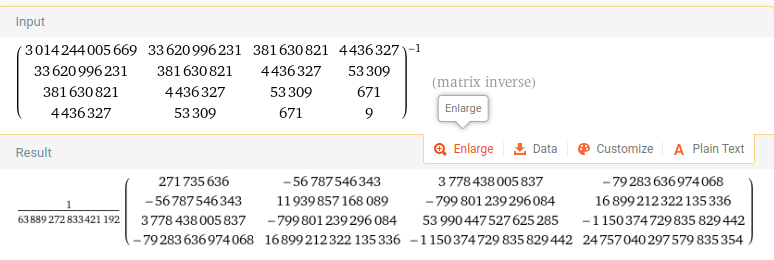
\includegraphics[width=\textwidth]{pictures/29-1.png}
  \end{center}
  Поэтому приведем программу на python:
  \begin{python}
  import numpy as np

  X = [4.0, 5.2, 6.1, 7.0, 7.9, 8.6, 8.9, 9.5, 9.9]
  F = [3.9, 5.0, 5.7, 6.5, 7.1, 7.6, 7.8, 8.1, 8.4]
  Z = list(map(lambda x: [x**3, x**2, x, 1], X))
  Z_np = np.array(Z)
  F_np = np.array(F)
  theta = np.linalg.inv(Z_np.T @ Z_np) @ Z_np.T @ F_np
  a, b, c, d = theta
  print(a, b, c, d)
  \end{python} и получим 
  \[(a, b, c, d) = (-0.00100145912636040, -0.0114849959500949, 1.07154905548792, -0.137289441132785) \]
  Вроде неплохо:
  \begin{python}
  import matplotlib.pyplot as plt

  plt.scatter(X, F, alpha=0.5)
  xseq = np.linspace(min(X), max(X), num=100)
  plt.plot(xseq, a * xseq**3 + b * xseq**2 + c * xseq + d,
           label=f'y={round(a, 3)}x^3 + {round(b, 3)}x^2 + {round(c, 3)}x + {round(d, 3)}')
  plt.legend()
  plt.show()
  \end{python}
  \begin{center}
  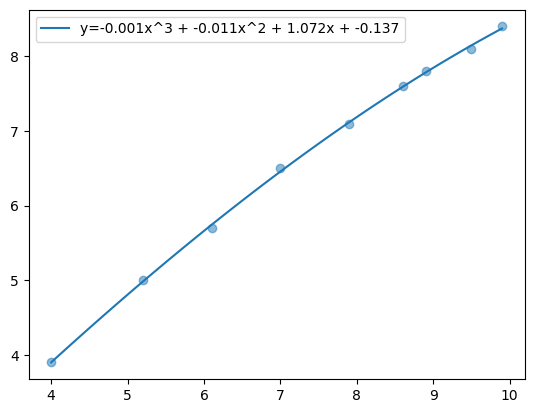
\includegraphics[width=0.5\textwidth]{pictures/29-2.png}
  \end{center}
  }
  \problem{
  Убедиться в том, что наиболее мощный критерий для различения двух простых гипотез о симметричном относитлтеьно нуля распределении набдюдаемой случайной величины $\xi \text{ } H_0 \text{  } \LL(\xi) = R[-a, a]$ и $H_1 \text{ } \LL(\xi) = \ND{0}{\sigma^2}$ ($a$ и $\sigma$ известны) имеет для больших выборок следующую асимптотическую форму 
  \[ \mathfrak{X_{1, a}^*} = \left\{ \sum_{i = 1}^n X_i^2 \le \frac{n}{3}a^2 + \zeta_a \frac{2a^2}{3}\sqrt{\frac{n}{5}}\right\}, \Phi(\zeta_a) = a\]
  }
  \guidance{
  Воспользоваться центральной предельной теоремой при отыскании распределения тестовой статистики.
  }
  \solution{}
  \problem{
  В последовательности независимых испытаний с двумя исходами вероятсноть ``успеха'' равна $p$. Построить критей проверки гипотезы $H_0 \text{ } p = 0$ против альтернативы $H_1 \text{ } p = 0.01$ и определить наименьший объем выборки, при котором вероятности ошибок 1-го и 2-го родов не превышают $0.01$.
  }
  \solution{}
  \problem{
  Имеется 2 гирьки с весами $\theta_1 $ и $\theta_2$. На одних и тех же весах сначала взвесили первую гирьку, затем вторую, а потом обе сразу. Найти оценку наименьших квадратов для $\theta_1$ и $\theta_2$ и несмещенную оценку дисперсии ошибки измерений. Проверьте гипотезы:
  а) $H_0 : \theta_1 = \theta_2$;
  б) $H_0 : 2\theta_1 = 3\theta_2$.
  }
  \solution{}
\end{document}